\chapter{System Implementation and Experimental Evaluation}
\label{chap:system-architecture}

This chapter describes the implemented monitoring system, the experimental setup, and the empirical results obtained on the fixed monitoring subset within the recorded time window. It focuses on operationalization rather than re-deriving the methodology: McNemar's test, evaluation metrics, and the manual selection procedure are defined in Chapter~\ref{ch:drift}, while prompt optimisation is discussed in Chapter~\ref{chap:prompt-optimisation}. Transient degradation behaviour is analysed separately in Chapter~\ref{chap:degradation-case-study}.

\section{Overview}
\label{sec:evaluation-pipeline-overview}

The implemented system separates three concerns: (i) dataset storage and stable row identifiers, (ii) batch execution with provider-specific adapters under a single shared request representation, and (iii) Langfuse-backed traces plus CSV snapshots for offline dashboard analytics. The evaluation implementation is maintained in a dedicated code repository; scheduled GitHub Actions workflows invoke \texttt{run\_eval.py} to submit batches, \texttt{poll\_and\_ingest.py} to download outputs and write Langfuse traces and scores, and \texttt{streamlit\_app/export\_langfuse\_csv.py} to export traces and scores into committed CSV files in the main evaluation repository. The same synchronization step then mirrors \texttt{streamlit\_app/} to the private dashboard repository from which the hosted Streamlit application is served.

\begin{itemize}
    \item \textbf{Dataset layer:} Langfuse stores the labelled reference benchmark and the fixed monitoring subset;
    \item \textbf{Execution layer:} scheduled GitHub Actions workflows execute repository scripts that submit, retrieve, and process benchmark and monitoring batches via provider APIs;
    \item \textbf{Trace and reporting layer:} Langfuse holds traces and scores; exported CSV snapshots are committed under \texttt{streamlit\_app/} in the main evaluation repository and mirrored to the private Streamlit deployment repository, so the dashboard does not query Langfuse on every page load in the default path.
\end{itemize}

Figure~\ref{fig:workflow-swimlane} summarizes orchestration across GitHub Actions, provider batch APIs, Langfuse, and the reporting path. Figure~\ref{fig:overall-system-architecture} gives a complementary repository-level diagram.

\begin{figure}[H]
    \centering
    \begin{adjustbox}{max width=\textwidth}
    \begin{tikzpicture}[
    node distance=4mm and 7mm,
    lbl/.style={font=\scriptsize\bfseries, anchor=east, text width=16mm, align=right}
    ]
    \node[lbl] (L1) at (0,0) {GitHub Actions};
    \node[figbox, right=9mm of L1] (g1) {\scriptsize Submit\\\texttt{run\_eval.py}};
    \node[figbox, right=of g1] (g2) {\scriptsize Retrieve\\\texttt{poll\_and\_ingest.py}};
    \node[figbox, right=of g2] (g3) {\scriptsize Sync\\\texttt{export\_langfuse\_csv.py}};
    \draw[figarrow] (g1) -- (g2);
    \draw[figarrow] (g2) -- (g3);

    \node[lbl] (L2) at (0,-1.9) {Providers};
    \node[figbox, right=9mm of L2] (p1) {\scriptsize Batch APIs\\OpenAI / Gemini / Claude};
    \node[figbox, right=of p1] (p2) {\scriptsize Raw\\JSONL outputs};

    \node[lbl] (L3) at (0,-3.8) {Langfuse};
    \node[figbox, right=9mm of L3] (lf1) {\scriptsize Datasets};
    \node[figbox, right=of lf1] (lf2) {\scriptsize Traces\\\& scores};

    \node[lbl] (L4) at (0,-5.7) {Reporting};
    \node[figbox, right=9mm of L4] (r1) {\scriptsize CSV commit to\\\texttt{llm-batch-eval}};
    \node[figbox, right=of r1] (r2) {\scriptsize Mirror to private\\\texttt{llm-eval-dashboard}};
    \node[figbox, right=of r2] (r3) {\scriptsize Hosted\\Streamlit app};

    \draw[figarrow] (p1) -- (p2);
    \draw[figarrow] (lf1) -- (lf2);
    \draw[figarrow] (r1) -- (r2);
    \draw[figarrow] (r2) -- (r3);
    \end{tikzpicture}
    \end{adjustbox}
    \caption{Orchestration swimlane (conceptual): scheduled jobs chain submit, retrieve or ingest, and CSV export; provider APIs return batch outputs ingested into Langfuse; exported dashboard artifacts are committed to the evaluation repository, mirrored to the private dashboard repository, and served there by the hosted Streamlit application.}
    \label{fig:workflow-swimlane}
\end{figure}

The key architectural decision is the separation between one-time subset construction and repeated monitoring. A manual full-benchmark run on \(N=1199\) labelled examples is used once to define the disagreement-based subset, whereas the recurring weekly loop operates only on the fixed \(n=300\) monitoring set. This keeps repeated evaluation inexpensive while preserving paired comparability across time.

\begin{figure}[H]
    \centering
    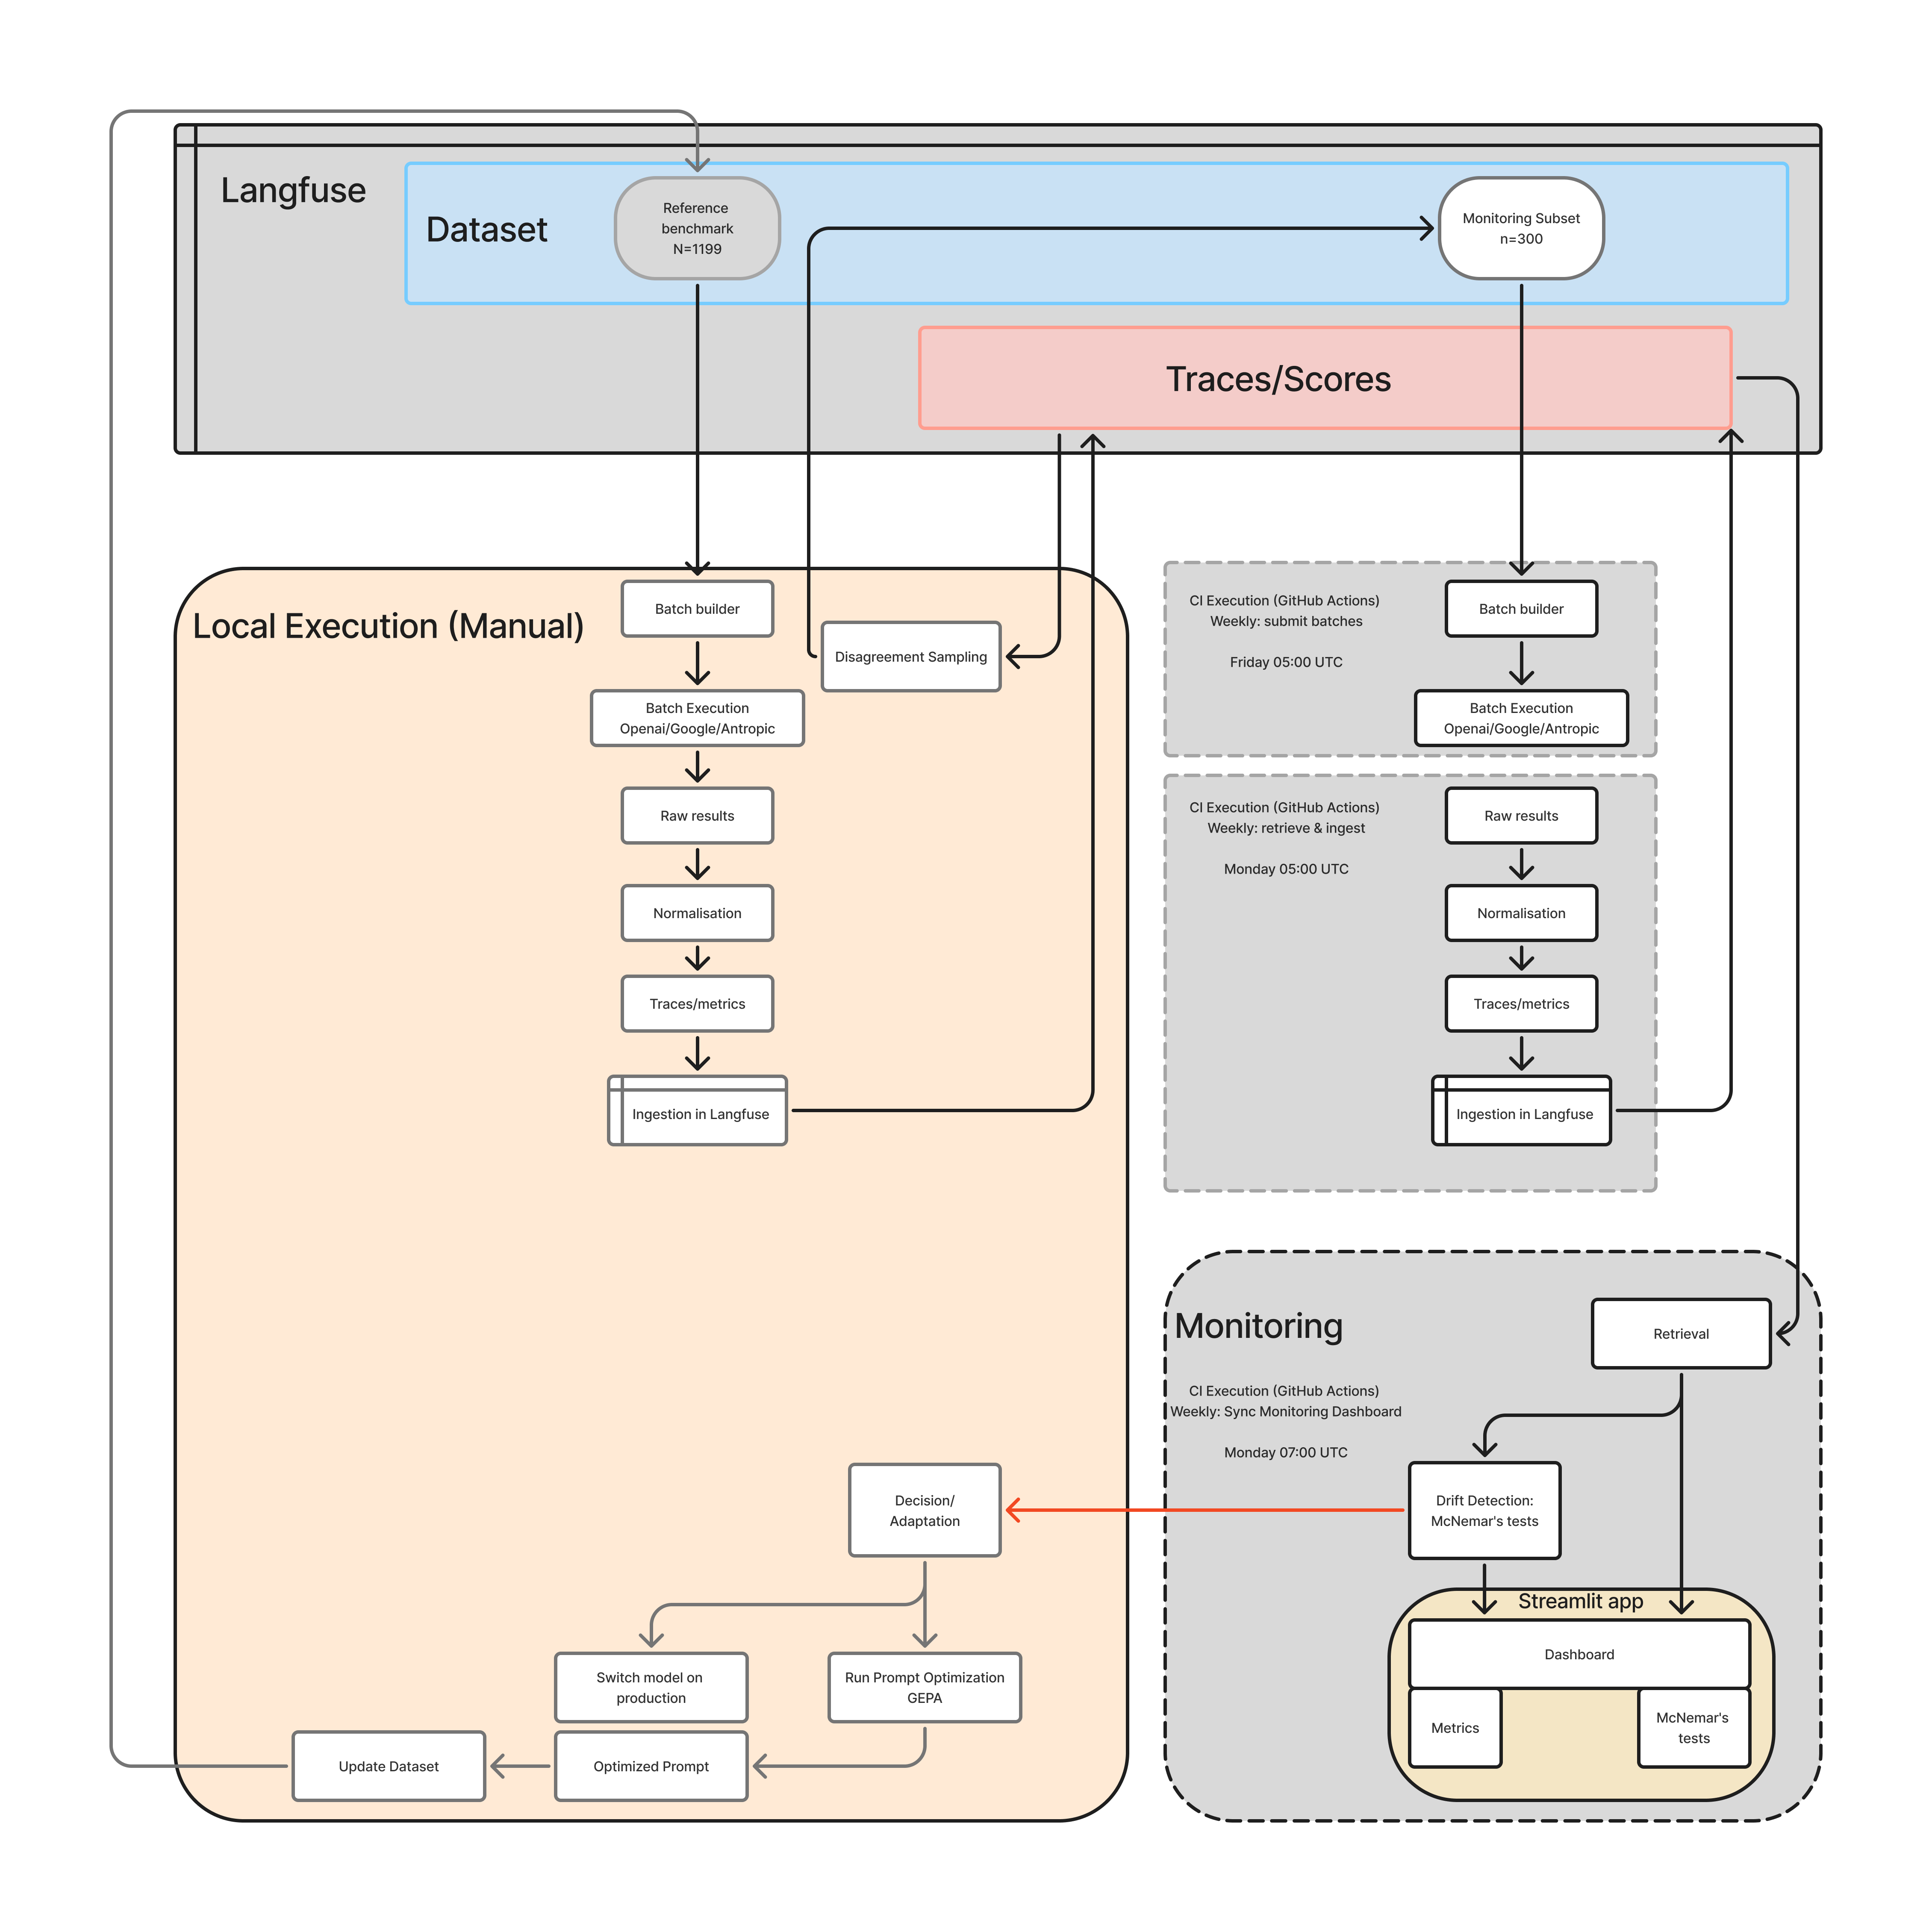
\includegraphics[width=\textwidth]{assets/System Architecture.png}
    \caption{Repository-level view: Langfuse stores datasets and ingested traces; scheduled GitHub Actions run batch scripts; monitoring analytics are exported as CSV artifacts in the main evaluation repository and mirrored to the private Streamlit dashboard repository for hosting.}
    \label{fig:overall-system-architecture}
\end{figure}

The same architecture therefore supports two run types:
\begin{itemize}
    \item \emph{Benchmark run:} a broader comparison on the full reference benchmark, with an overall batch cost of approximately USD~90 for one full benchmark pass;
    \item \emph{Monitoring run:} a recurring paired evaluation on the fixed 300-example subset, with an overall batch cost of approximately USD~20 for one full monitoring pass.
\end{itemize}

The benchmark run defines the monitoring instrument; weekly subset runs supply the longitudinal evidence analysed later in this chapter.

\section{Implemented Monitoring Pipeline}

\subsection{Data sources and request normalization}
\label{sec:dataset-storage}

The implementation uses two Langfuse datasets:
\begin{itemize}
    \item \textbf{Reference benchmark} (\(N=1199\)): \href{https://cloud.langfuse.com/project/cmkqnvv3z016aad08kqtjim2n/datasets/cmlfi3uo0003yad07e75cd7e3}{Langfuse link};
    \item \textbf{Monitoring subset} (\(n=300\)): \href{https://cloud.langfuse.com/project/cmkqnvv3z016aad08kqtjim2n/datasets/cmmjjduz501c6ad07vbuln8m8/items}{Langfuse link}.
\end{itemize}

Langfuse acts as the single source of truth for both dataset scales. Each row carries a stable \texttt{custom\_id}, reused end-to-end across batch submission, raw result files, ingested traces, CSV exports, and statistical analyses.

Each dataset row includes the campaign description, post text, transcription, hashtags, media references, frame references where applicable, and the binary ground-truth label \texttt{campaign\_relevant}. Reusing the same schema for both the \(N=1199\) benchmark and the \(n=300\) monitoring subset ensures that the smaller set is a frozen projection of the original benchmark onto informative disagreement cases, not a separate task definition.

The 300-example monitoring dataset is selected once from the full benchmark and then held fixed. This immutability makes per-example histories meaningful and ensures that paired McNemar comparisons are not confounded by changes in sample composition.

\paragraph{Loader and canonical request body.}
Rows are normalized in code to a shared structure \texttt{\{custom\_id, body, campaign\_relevant\}}. The \texttt{body} follows an OpenAI-style \emph{Responses} request object: a template (from \texttt{config/request\_template.json} or the first row of a template CSV) is merged with per-item multimodal \texttt{input} when loading from Langfuse; CSV mode parses a Python literal \texttt{body} column per row. The same representation is passed to all provider adapters, so only transport and provider-specific constraints differ downstream. A local CSV path remains supported so the frozen subset can be replayed without live Langfuse access.

After each run, outputs are written back into Langfuse as traces. Each trace stores the normalized response, provider and model identifiers, token usage, monetary cost, and derived scores. Langfuse therefore serves both as the registry of evaluation instances and as the persistent log of how each monitored model behaved on each instance over time.

\subsection{Workflow orchestration and batch submission}
\label{sec:batch-process}

The orchestrator \texttt{run\_eval.py} loads the eval subset, optionally ensures Gemini image uploads when any Gemini model is selected, dispatches each model to the corresponding \texttt{batch\_*.py} adapter, and writes a run manifest \texttt{data/batch\_ids.json} containing \texttt{run\_id}, \texttt{subset\_size}, and per-model batch identifiers. Between runs the workspace may clear \texttt{data/results/} before submission. Scheduled monitoring uses three GitHub Actions workflows (all times UTC): \textbf{Friday 05:00} submit batches; \textbf{Monday 05:00} poll, download, and ingest; \textbf{Monday 07:00} export Langfuse traces and scores to CSV under \texttt{streamlit\_app/}, commit those CSV snapshots back to the main evaluation repository \texttt{gocomo/llm-batch-eval}, and then mirror the full \texttt{streamlit\_app/} tree to the separate private dashboard repository \texttt{GeorgiiBurdinComo/llm-eval-dashboard}. The submit job saves \texttt{data/batch\_ids.json} to the Actions cache under a key derived from the submit run id; the retrieve job restores the latest matching cache entry so the retrieve workflow does not depend on downloading the submit workflow's artifact by name.

Chronologically, one evaluation cycle consists of:
\begin{enumerate}
    \item load the target split via the dataset loader (Langfuse dataset or CSV);
    \item merge each row with the shared template into the canonical \texttt{body};
    \item if any Gemini model is run, upload remote image URLs to the Gemini Files API and refresh \texttt{data/gemini\_image\_cache.json} as needed;
    \item serialize requests through the provider-specific batch adapter and submit asynchronous batch jobs;
    \item persist returned batch identifiers in \texttt{data/batch\_ids.json};
    \item after completion, retrieve outputs into \texttt{data/results/} and pass them to ingestion for Langfuse traces and scores;
    \item on a separate schedule, export Langfuse data to committed CSVs for the dashboard.
\end{enumerate}

This split reflects asynchronous provider batch semantics: submission, retrieval or ingestion, and dashboard synchronization are decoupled because results are not available immediately after submission. Figure~\ref{fig:weekly-monitoring-loop} shows the weekly schedule and main artifacts; Figure~\ref{fig:artifact-flow} shows the data artifact chain.

\begin{figure}[H]
    \centering
    \begin{adjustbox}{max width=0.92\textwidth}
    \begin{tikzpicture}[
    node distance=8mm and 18mm
    ]
    
    \node[figbox] (submitTime) {Friday\\05{:}00 UTC};
    \node[figbox, below=of submitTime] (submitWf) {Github\\Workflow\\Submit\\Drift\\Monitoring};
    \node[figbox, below=of submitWf] (runEval) {Repository\\Batch\\Scripts};
    \node[figbox, below=of runEval] (batchIds) {Batch IDs\\\texttt{data/batch\_ids.json}};
    
    \node[figbox, right=32mm of submitTime] (retrieveTime) {Monday\\05{:}00 UTC};
    \node[figbox, below=of retrieveTime] (retrieveWf) {Github\\Workflow\\Retrieve\\\& Ingest};
    \node[figbox, below=of retrieveWf] (pollIngest) {Poll\\\& Download\\Results};
    \node[figbox, below=of pollIngest] (results) {Result Files\\\texttt{data/results/*.jsonl}};
    \node[figbox, below=of results] (traces) {Ingest\\Langfuse\\Traces\\/ Scores};
    
    \node[figbox, right=32mm of retrieveTime] (syncTime) {Monday\\07{:}00 UTC};
    \node[figbox, below=of syncTime] (syncWf) {Github\\Workflow\\Sync\\Dashboard};
    \node[figbox, below=of syncWf] (exportCsv) {Commit CSVs to\\\texttt{llm-batch-eval}};
    \node[figbox, below=of exportCsv] (dashboard) {Mirror\\\texttt{streamlit\_app/} to\\private \texttt{llm-eval-dashboard}};
    
    \draw[figarrow] (submitTime) -- (submitWf);
    \draw[figarrow] (submitWf) -- (runEval);
    \draw[figarrow] (runEval) -- (batchIds);
    
    \draw[figarrow] (retrieveTime) -- (retrieveWf);
    \draw[figarrow] (retrieveWf) -- (pollIngest);
    \draw[figarrow] (pollIngest) -- (results);
    \draw[figarrow] (results) -- (traces);
    
    \draw[figarrow] (syncTime) -- (syncWf);
    \draw[figarrow] (syncWf) -- (exportCsv);
    \draw[figarrow] (exportCsv) -- (dashboard);
    
    \draw[figarrow] (batchIds) -- (retrieveWf);
    \draw[figarrow] (traces) -- (syncWf);
    
    \end{tikzpicture}
    \end{adjustbox}
    \caption{Weekly schedule (UTC): submit on Friday; retrieve, poll, and ingest on Monday morning; then commit exported CSV snapshots to the main evaluation repository and mirror the Streamlit application to the separate private dashboard repository two hours later. \texttt{data/batch\_ids.json} is passed from submit to retrieve via the Actions cache.}
    \label{fig:weekly-monitoring-loop}
\end{figure}

The concrete set of monitored models and token prices used for cost accounting is defined in \texttt{config/models.yaml} and summarized in Table~\ref{tab:monitored-models}.

\begin{table}[htbp]
\centering
\caption{LLM models monitored in this study, grouped by provider.}
\label{tab:monitored-models}
\begin{tabular}{ll}
\toprule
\textbf{Provider} & \textbf{Models} \\
\midrule
OpenAI   & \texttt{gpt-5.4-2026-03-05}, \texttt{gpt-5.2}, \texttt{gpt-5.1}, \texttt{gpt-5}, \\
         & \texttt{gpt-5-mini}, \texttt{gpt-5-nano}, \texttt{gpt-4.1-mini}, \texttt{gpt-4.1-nano} \\
Gemini   & \texttt{gemini-2.5-flash}\\
Claude   & \texttt{claude-sonnet-4-6}, \texttt{claude-sonnet-4-5}, \texttt{claude-haiku-4-5} \\
\bottomrule
\end{tabular}
\end{table}

\subsection{Provider-specific batch adapters}
\label{sec:provider-adapters}

The logical task is provider-invariant: every request asks for the same campaign-relevance classification under the same structured output constraints. Differences are isolated in the batch adapters. Table~\ref{tab:provider-adapters} summarizes how each backend maps the shared \texttt{body} to its native batch format.

\begin{table}[htbp]
\centering
\footnotesize
\caption{Provider adapters over the shared request \texttt{body} (multimodal \texttt{input} + JSON schema for \texttt{campaign\_relevant}).}
\label{tab:provider-adapters}
\begin{adjustbox}{max width=\linewidth}
\begin{tabular}{p{1.8cm}p{3.6cm}p{3.2cm}p{3.5cm}}
\toprule
\textbf{Provider} & \textbf{Batch wire format} & \textbf{Structured output} & \textbf{Images / ids} \\
\midrule
OpenAI & JSONL: \texttt{POST} \texttt{/v1/responses} per row & \texttt{text.format} JSON schema & Multimodal \texttt{input}; image URLs \\
Gemini & Native batch JSONL; uploaded file & \texttt{responseSchema} + JSON MIME type & URLs $\rightarrow$ Files \texttt{fileUri}; cache TTL $\approx$47\,h; rows may be skipped if URLs missing \\
Claude & Staging JSONL + Messages Batches & Anthropic \texttt{output\_config} schema & Sanitized \texttt{custom\_id}; remap on download \\
\bottomrule
\end{tabular}
\end{adjustbox}
\end{table}

\paragraph{Gemini image preprocessing.}
Gemini batch lines require uploaded file URIs instead of remote HTTP image URLs. The helper \texttt{upload\_gemini\_images.py} downloads each distinct URL, uploads via the Gemini Files API, and records URI, file name, and upload timestamp per URL in \texttt{data/gemini\_image\_cache.json}. Entries older than the TTL are ignored when building batches so stale file handles are not reused.

The structural differences are easiest to see in abbreviated examples:

\begin{lstlisting}[
        caption={Batch entry formats across providers.},
        label={lst:batch-provider-structures},
        frame=single,
        basicstyle=\ttfamily\small,
        breaklines=true
        ]
        === OpenAI ===
        {"custom_id":"...", "method":"POST", "url":"/v1/responses",
         "body":{
           "input":[...],
           "text":{"format":{"type":"json_schema"}}
         }}
        
        === Gemini ===
        {"key":"...", "request":{
         "systemInstruction":{"parts":[{"text":"..."}]},
         "contents":[{"role":"user","parts":[
           {"text":"..."},
           {"fileData":{"fileUri":"..."}}
         ]}],
         "generationConfig":{
           "responseMimeType":"application/json",
           "responseSchema":{...}
         }}}
        
        === Claude (staging JSONL) ===
        {"custom_id":"...", "sanitized_id":"...",
         "body":{
           "input":[...],
           "text":{"format":{"type":"json_schema"}}
         }}
        \end{lstlisting}

Across all three providers, the parsed prediction is aligned with the same minimal schema for monitoring:
\[
\{\texttt{campaign\_relevant},\; \texttt{relevancy\_reasoning}\}.
\]

\subsection{Artifacts and cross-step data flow}
\label{sec:artifacts-data-flow}

Table~\ref{tab:artifact-inventory} lists the main files and stores. Figure~\ref{fig:artifact-flow} shows how they chain from dataset rows to dashboard inputs.

\begin{table}[htbp]
\centering
\footnotesize
\caption{Main artifacts and handoffs in the evaluation pipeline.}
\label{tab:artifact-inventory}
\begin{adjustbox}{max width=\linewidth}
\begin{tabular}{p{2.7cm}p{2.2cm}p{2.2cm}p{2.1cm}p{3.2cm}}
\toprule
\textbf{Artifact} & \textbf{Producer} & \textbf{Consumer} & \textbf{Storage} & \textbf{Purpose} \\
\midrule
\texttt{data/batch\_ids.json} & \texttt{run\_eval.py} & \texttt{poll\_and\_ingest.py} & Actions cache + workspace & Run manifest (batch ids per model) \\
\texttt{batches/*.jsonl} & \texttt{batch\_*.py} & Provider batch APIs & Repository & Provider batch inputs \\
\texttt{data/gemini\_image\_cache.json} & \texttt{upload\_gemini\_images.py} & \texttt{batch\_gemini.py} & Repository & URL to Files API URI \\
\texttt{data/results/*.jsonl} & Provider download & Ingestion & Workspace & Raw outputs \\
Langfuse traces \& scores & Ingestion & Export, app & Langfuse cloud & Join keys, tags, metrics \\
\texttt{langfuse\_*.csv} & Export script & Hosted Streamlit app & \texttt{streamlit\_app/} in \texttt{llm-batch-eval}, then mirrored to \texttt{llm-eval-dashboard} & Dashboard snapshots \\
\bottomrule
\end{tabular}
\end{adjustbox}
\end{table}

\begin{figure}[H]
    \centering
    \begin{adjustbox}{max width=\textwidth}
    \begin{tikzpicture}[
    node distance=2mm
    ]
    \node[figboxsmall] (reference) {Langfuse\\or CSV\\rows};
    \node[figboxsmall, right=of reference] (load) {\texttt{load\_dataset}};
    \node[figboxsmall, right=of load] (submit) {\texttt{run\_eval}};
    \node[figboxsmall, right=of submit] (ids) {\texttt{batch\_ids}\\\texttt{.json}};
    \node[figboxsmall, right=of ids] (raw) {Raw\\\texttt{results/}};
    \node[figboxsmall, right=of raw] (traces) {Langfuse\\traces};
    \node[figboxsmall, right=of traces] (csv) {CSV in\\\texttt{llm-batch-eval}};
    \node[figboxsmall, right=of csv] (mirror) {Mirror to\\private repo};
    \node[figboxsmall, right=of mirror] (dash) {Hosted\\Streamlit};
    \draw[figarrow] (reference) -- (load);
    \draw[figarrow] (load) -- (submit);
    \draw[figarrow] (submit) -- (ids);
    \draw[figarrow] (ids) -- (raw);
    \draw[figarrow] (raw) -- (traces);
    \draw[figarrow] (traces) -- (csv);
    \draw[figarrow] (csv) -- (mirror);
    \draw[figarrow] (mirror) -- (dash);
    \end{tikzpicture}
    \end{adjustbox}
    \caption{Artifact flow: normalized dataset rows drive batch submission and a manifest; retrieved JSONL is ingested into Langfuse; paginated API export produces CSV snapshots in the main evaluation repository, which are then mirrored to the private dashboard repository that serves the hosted Streamlit application.}
    \label{fig:artifact-flow}
\end{figure}

\subsection{Ingestion, Scoring, and Exports}
\label{sec:metrics-dashboard}

Once raw batch outputs have been retrieved, the monitoring layer converts them into a common analytical representation. For each output line, ingestion performs five steps:
\begin{enumerate}
    \item normalize the provider-specific response;
    \item extract \texttt{campaign\_relevant} and join it to the ground truth via \texttt{custom\_id};
    \item compute token usage from the provider-specific usage fields;
    \item convert token usage into USD cost via \texttt{config/models.yaml};
    \item write the resulting Langfuse trace together with derived scores and metadata.
\end{enumerate}

The full batch-API price table for all monitored models is provided in Appendix~\ref{app:batch-pricing-table} as Table~\ref{tab:batch-pricing-examples}.

Three trace-level scores are central for the later evaluation:
\begin{itemize}
    \item \texttt{accuracy} \(\in \{0,1\}\), indicating per-example correctness;
    \item \texttt{error\_type}, distinguishing true positives, false positives, true negatives, and false negatives;
    \item \texttt{cost\_usd}, giving the realized dollar cost of the request.
\end{itemize}

From \texttt{error\_type}, precision, recall, and F1 are computed per run on $\mathcal{D}_n$ as in Section~\ref{sec:classification-metrics}. The same traces feed drift tests and corrective-action comparisons.

\subsection{Dashboard and Analysis Surfaces}

The Streamlit dashboard does not query Langfuse on every interaction in the default path. The synchronization workflow runs \texttt{export\_langfuse\_csv.py}, which paginates the Langfuse public API for traces and scores over a configured time window, flattens nested fields, retains columns used by the app, and writes \texttt{streamlit\_app/langfuse\_traces.csv} and \texttt{langfuse\_scores.csv}. Those files are committed to the main evaluation repository \texttt{gocomo/llm-batch-eval}; the same workflow then mirrors \texttt{streamlit\_app/} to the private dashboard repository \texttt{GeorgiiBurdinComo/llm-eval-dashboard}, from which the hosted Streamlit application is served. This keeps analytics reproducible and avoids embedding long-lived Langfuse credentials in the hosted app.

The dashboard exposes three main tabs. The overview tab shows per-model accuracy over time together with aggregated cost summaries from \texttt{cost\_usd}; the McNemar tab reports paired contingency tables and exact p-values for selected run pairs; and the utility-function tab combines accuracy and cost through a tunable penalty parameter $\lambda$ to support deployment trade-off analysis. Screenshots of the paired-drift and metric--cost or utility views are in Sections~\ref{sec:drift-results} and~\ref{sec:cost-aware-comparison}.

Exported CSVs also feed notebooks for inspection beyond the dashboard.
\FloatBarrier

\section{Experimental Setup}
\label{sec:experimental-design}

Experiments use the full benchmark \(\mathcal{D}_N\) (\(N=1199\)) and the frozen subset \(\mathcal{D}_n\) (\(n=300\)) from Chapter~\ref{ch:data}. The model roster is \texttt{config/models.yaml} (Table~\ref{tab:monitored-models}). Each run yields one trace per example and a paired correctness vector for McNemar comparisons (Section~\ref{sec:mcnemar-section}).

The empirical results are reported in four parts: the instantiated monitoring subset and its baseline snapshot; longitudinal monitoring on the fixed subset; candidate comparison for corrective action; and the implemented prompt-recovery branch. Drift alerts, manual comparison, and optional prompt recovery follow Chapter~\ref{ch:drift}; Figure~\ref{fig:run-decision-logic} sketches the operational workflow without restating the formal test.
\FloatBarrier
\begin{figure}[H]
    \centering
    \begin{adjustbox}{max width=0.92\textwidth}
    \begin{tikzpicture}[
    >=Latex,
    node distance=10mm and 16mm
    ]
    
    \node[figbox] (baseline) {Baseline\\Run\\Metrics};
    \node[figbox, right=of baseline] (newrun) {New\\Run\\Metrics};
    
    \node[figbox, below=of newrun] (drift) {DriftTest\\McNemar on fixed\\300-example subset};
    
    \node[figbox, left=25mm of drift] (deploy) {Deploy\\Current\\Setup};
    \node[figbox, right=25mm of drift] (metriccost) {Compare\\metrics + cost\\};
    
    \node[figbox, below=of metriccost] (decision) {Decision\\Node};
    \node[figbox, left=of decision] (switch) {Switch\\Model};
    \node[figbox, right=of decision] (gepa) {Run\\GEPA};
    \node[figbox, below=of gepa] (reeval) {Re\\Evaluate};
    
    \draw[figarrow] (baseline) -- (drift);
    \draw[figarrow] (newrun) -- (drift);
    
    \draw[figarrow] (drift) -- node[above, font=\scriptsize]{no drift} (deploy);
    \draw[figarrow] (drift) -- node[above, font=\scriptsize]{drift} (metriccost);
    
    \draw[figarrow] (metriccost) -- (decision);
    \draw[figarrow] (decision) -- (switch);
    \draw[figarrow] (decision) -- (gepa);
    \draw[figarrow] (gepa) -- (reeval);
    
    \draw[figarrow] (reeval.west) |- (metriccost.south);
    
    \end{tikzpicture}
    \end{adjustbox}
    \caption{Decision logic after a monitoring run. Drift is tested on the fixed 300-example subset. If no statistically significant degradation is detected, the current setup is retained. If degradation is detected, corrective actions are compared using accuracy, precision, recall, F1, and cost. This may lead either to model switching or to prompt optimisation with subsequent re-evaluation.}
    \label{fig:run-decision-logic}
    \end{figure}
    \FloatBarrier

\section{Results}

\subsection{Baseline and Instantiated Monitoring Subset}
\label{sec:baseline-subset}

The first empirical step is the one-time full-benchmark run on the \(N=1199\) reference dataset. Its purpose is to establish initial per-model behaviour on the full benchmark and to identify those examples on which model decisions diverge. These disagreement cases are the operational signal used to instantiate the smaller monitoring subset described in Chapter~\ref{ch:data}.

This step therefore produces two outputs. First, it yields a full benchmark record that can be reused for broad model comparison. Second, it produces the fixed \(n=300\) disagreement-based monitoring set that is stored as a separate Langfuse dataset and then frozen for all later paired analyses.

Once created, the monitoring subset becomes the empirical backbone of the thesis. All later drift statistics, dashboard views, and adaptation decisions are computed on this fixed set. The recurring evidence in the remainder of the chapter therefore comes from repeated reuse of the same 300 difficult cases rather than from re-sampling.

Table~\ref{tab:phase1-baseline-snapshot} gives a compact baseline after the subset is frozen: aggregate accuracy, precision, recall, and F1 for two API models that participate in the disagreement construction and in later monitoring. Counts $n$ refer to scored examples in that export, with one missing score for \texttt{gpt-4.1-mini}. Full-benchmark $\mathcal{D}_N$ aggregates are produced in the same way but are not duplicated here; the empirical focus is the frozen hard-case subset and comparable scalar summaries on~$\mathcal{D}_n$.

\begin{table}[htbp]
    \centering
    \caption{Baseline snapshot: classification metrics on the frozen monitoring subset after construction (batch export, last score day 2026-03-28).}
    \label{tab:phase1-baseline-snapshot}
    \begin{tabular}{lccccc}
        \toprule
        Model & $n$ & Accuracy & Precision & Recall & F1 \\
        \midrule
        \texttt{gpt-4.1-mini} & 299 & {\csname benchgpt41miniaccuracy\endcsname} & {\csname benchgpt41miniprecision\endcsname} & {\csname benchgpt41minirecall\endcsname} & {\csname benchgpt41minif1\endcsname} \\
        \texttt{gpt-4.1-nano}  & 300 & {\csname benchgpt41nanoaccuracy\endcsname} & {\csname benchgpt41nanoprecision\endcsname} & {\csname benchgpt41nanorecall\endcsname} & {\csname benchgpt41nanof1\endcsname} \\
        \bottomrule
    \end{tabular}
\end{table}

\subsection{Longitudinal Monitoring Results}
\label{sec:drift-results}

This subsection evaluates whether repeated runs on the fixed monitoring subset reveal meaningful temporal changes in model behaviour. Because the subset is held constant, any change in the paired counts \((b,c)\) can be attributed to changed model predictions rather than to a changed sample.

\begin{table}[htbp]
    \centering
    \caption{McNemar table for \texttt{gpt-5} between 8~March~2026 and 10~March~2026 on $\mathcal{D}_n$.}
    \label{tab:mcnemar_gpt5}
    \begin{tabular}{c|cc}
        & 2026-03-10 correct & 2026-03-10 wrong \\
        \hline
        2026-03-08 correct & 291 & 0 \\
        2026-03-08 wrong   & 0   & 9 \\
    \end{tabular}
\end{table}

\begin{table}[htbp]
    \centering
    \caption{McNemar table for \texttt{gpt-5.1-mini} between 8~March~2026 and 10~March~2026 on $\mathcal{D}_n$.}
    \label{tab:mcnemar_gpt5mini}
    \begin{tabular}{c|cc}
        & 2026-03-10 correct & 2026-03-10 wrong \\
        \hline
        2026-03-08 correct & 269 & 13 \\
        2026-03-08 wrong   & 7   & 11 \\
    \end{tabular}
\end{table}

Two monitored examples illustrate the range of outcomes. For \texttt{gpt-5}, the run pair from 8~March~2026 to 10~March~2026 yields the contingency table in Table~\ref{tab:mcnemar_gpt5}. The discordant counts are \((b,c)=(0,0)\), so no monitored instance changed correctness between the two dates. In operational terms, this is the strongest possible evidence of short-term stability on the subset.

For \texttt{gpt-5.1-mini}, the corresponding run pair in Table~\ref{tab:mcnemar_gpt5mini} yields \((b,c)=(13,7)\): 20 instances change status (13 regressions, 7 recoveries). The one-sided test does not reach \(\alpha=0.05\); numerically, accuracy falls but the alert rule in Chapter~\ref{ch:drift} is not met.

\begin{figure}[htbp]
    \centering
    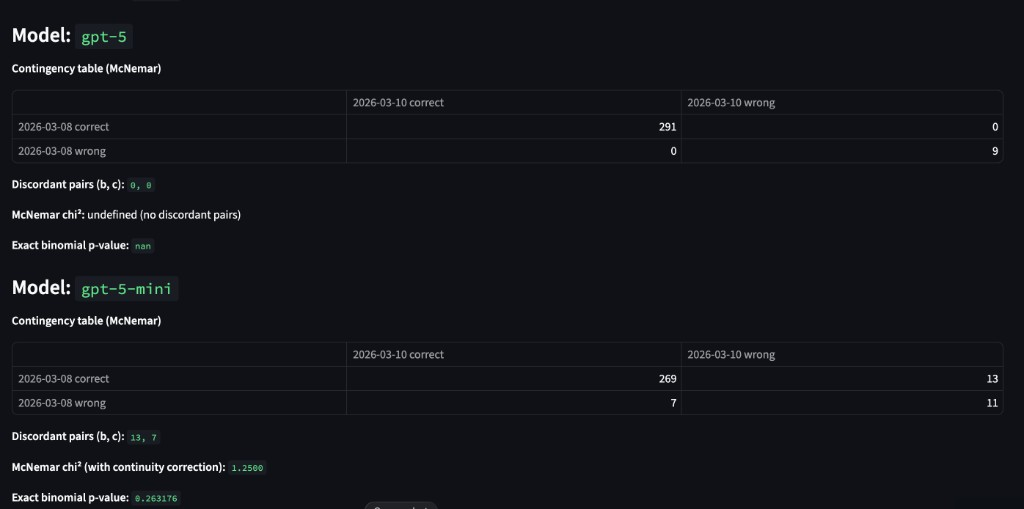
\includegraphics[width=\linewidth]{assets/Screenshot_2026-03-13_at_18.12.49-ab3bb230-c6fd-429c-b7d7-1a9af08a4170.png}
    \caption{Streamlit paired-drift view for \texttt{gpt-5} (top: $(b,c)=(0,0)$) and \texttt{gpt-5.1-mini} (bottom: $(b,c)=(13,7)$).}
    \label{fig:mcnemar-dashboard}
\end{figure}

The paired view distinguishes complete stability from mixed regressions and recoveries.

\subsection{Candidate Comparison for Corrective Action}
\label{sec:cost-aware-comparison}

This result block asks how a monitoring system should support choice among candidate corrective actions once predictive quality and cost are both visible. Each monitored run yields empirical accuracy, precision, recall, and F1 on the fixed subset together with mean per-request cost (Chapter~3). Operators compare candidates manually: some campaigns tolerate more false positives than others, so no single ranking rule is imposed in the experiments reported here.

\paragraph{Authoritative export.}
The \textbf{single authoritative numeric panel} for corrective-action comparison in this thesis is Table~\ref{tab:model-metrics-snapshot}. It is generated from \texttt{assets/metrics\_export/} (see \texttt{metrics\_wide.csv} and \texttt{export\_meta.json}) and input via \texttt{metrics\_tabular.tex}. The table lists confusion counts $(\mathrm{tp},\mathrm{fp},\mathrm{tn},\mathrm{fn})$, threshold-based metrics, specificity, balanced accuracy, and PR--AUC for each candidate in one snapshot.

Mean USD cost per request is \emph{not} in that static file; it is read from Langfuse traces as in Section~\ref{sec:metrics-dashboard}. For example, \texttt{gpt-4.1-mini} shows exported subset accuracy {\csname benchgpt41miniaccuracy\endcsname} versus \texttt{gpt-4.1-nano} {\csname benchgpt41nanoaccuracy\endcsname} on that snapshot. Figures~\ref{fig:metrics-by-model-bars} and~\ref{fig:utility-overview} support the same comparison visually: the former is a compact offline bar chart of the same metric dimensions across models on a fixed slice; the latter is the Streamlit dashboard view used to inspect trade-offs across date windows and model sets together with cost. The result is a \textbf{decision surface}---multiple metrics and cost---rather than a single universally best model. That matches the need to compare continued deployment, model switching, and prompt recovery under campaign-specific priorities.

\begin{figure}[htbp]
    \centering
    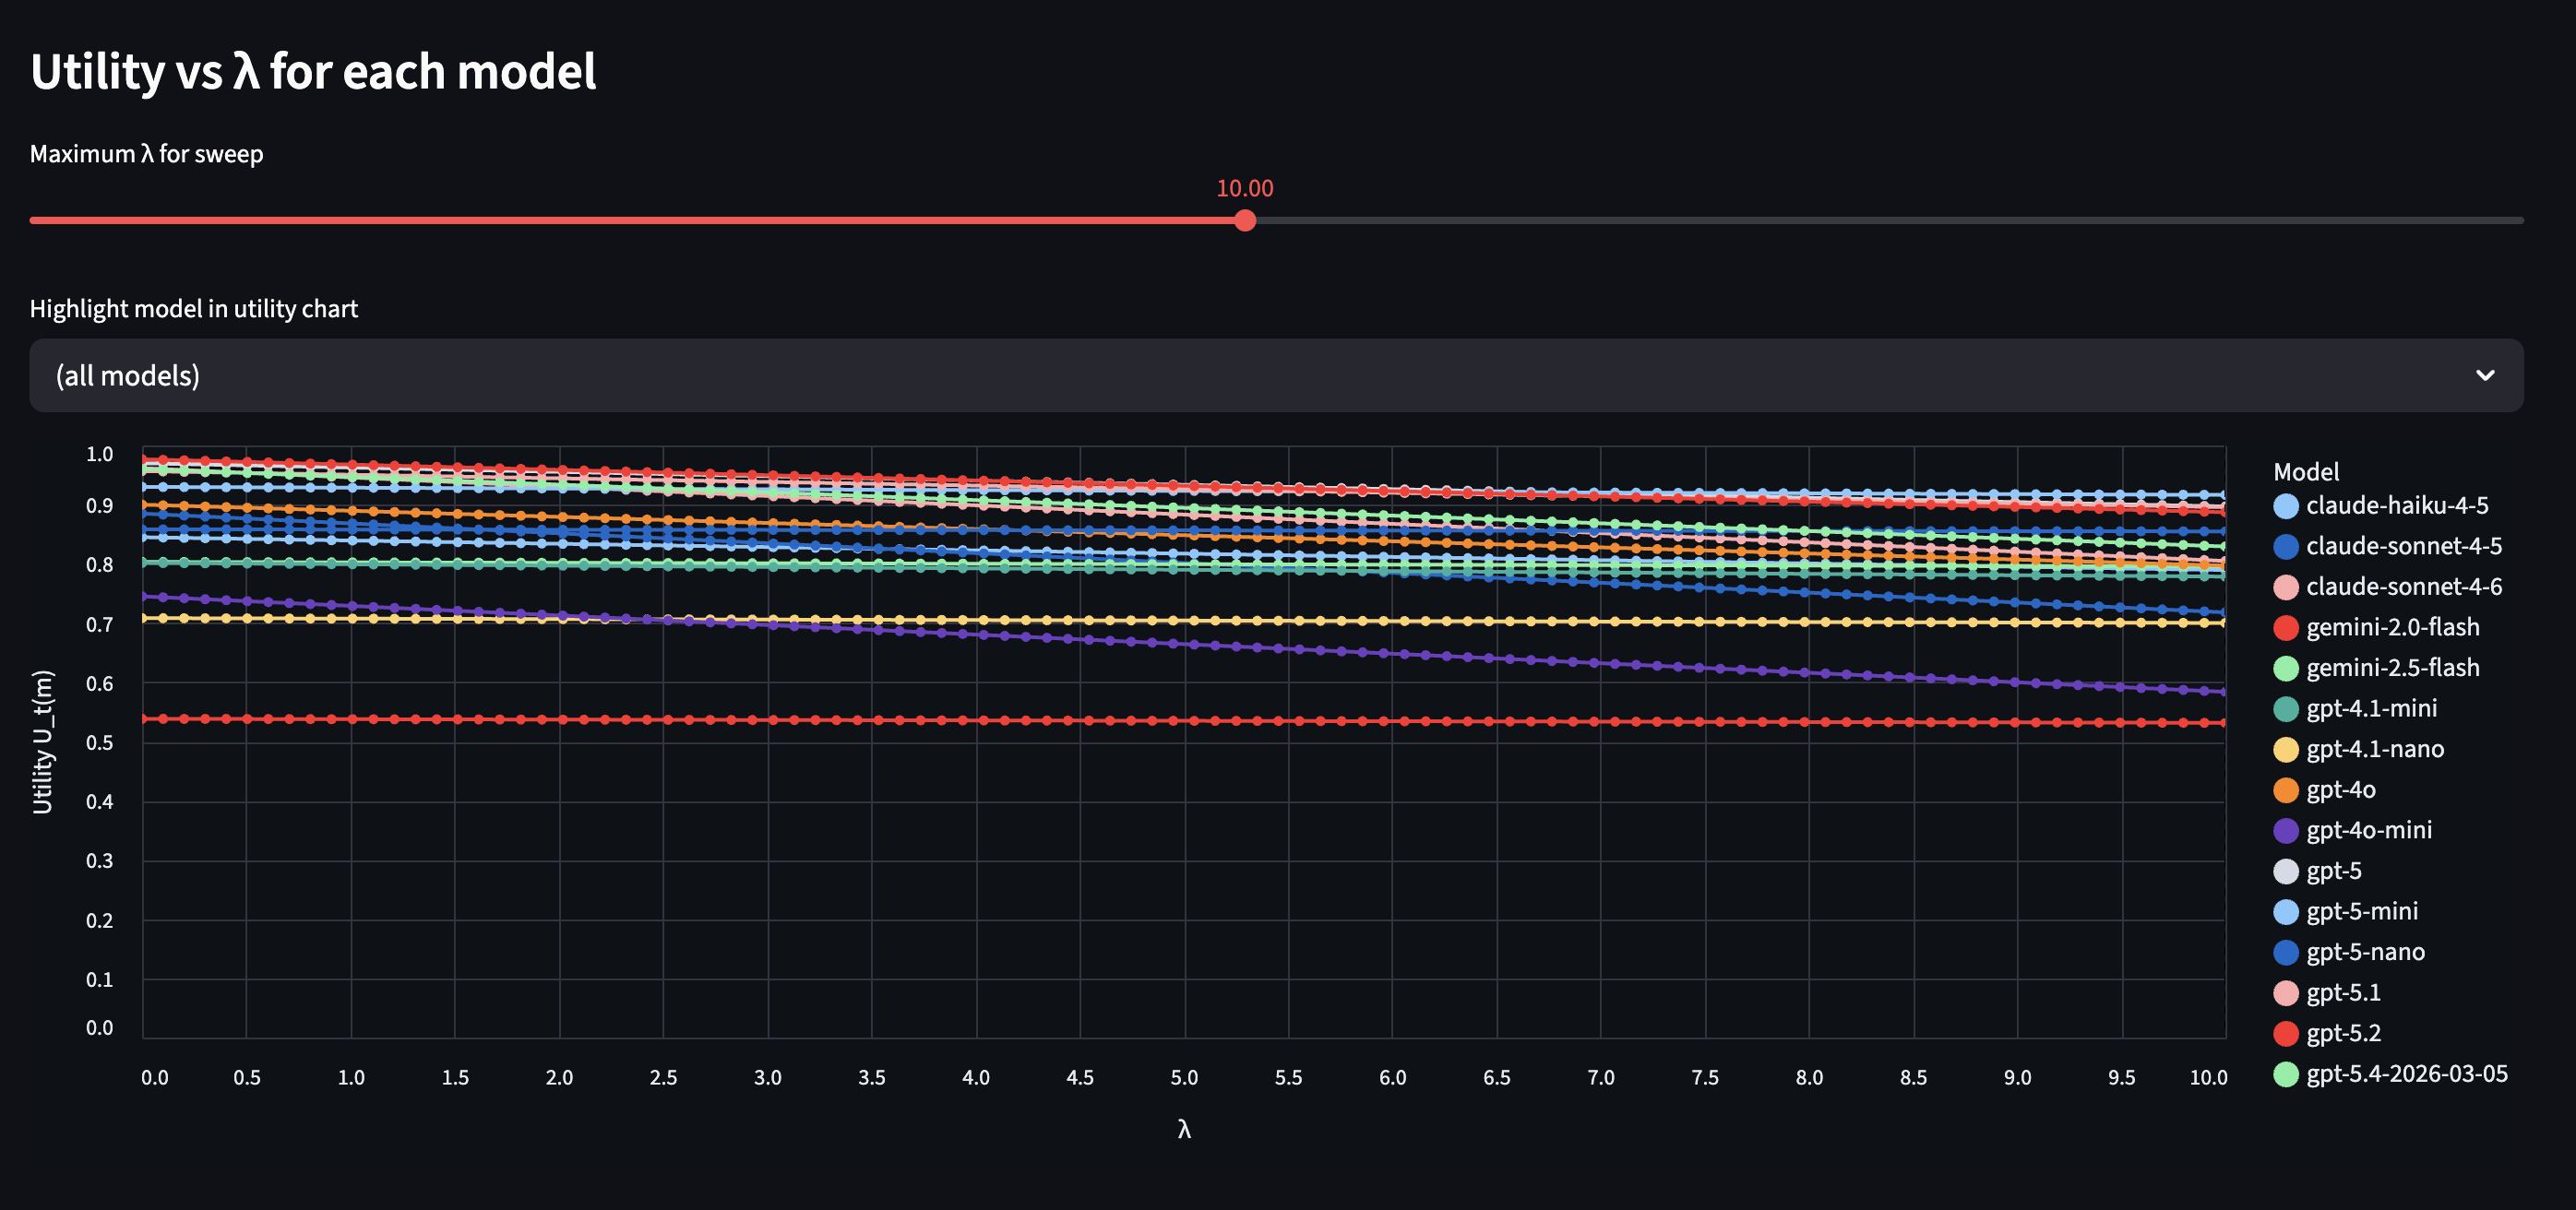
\includegraphics[width=\linewidth]{assets/utility_overview.png}
    \caption{Streamlit metric--cost comparison: accuracy, precision, recall, F1, mean cost (Chapter~\ref{ch:drift}).}
    \label{fig:utility-overview}
\end{figure}


\begin{table}[htbp]
    \centering
    \footnotesize
    \begin{adjustbox}{max width=\linewidth}
    % Auto-generated — last score day 2026-03-28
% % Auto-generated — last score day 2026-03-28
% % Auto-generated — last score day 2026-03-28
% \input{metrics_tabular.tex} inside your table environment
\begin{tabular}{lrrrrrrrrrrrr}
\toprule
model & n & tp & fp & tn & fn & accuracy & precision & recall & f1 & specificity & balanced\_accuracy & pr\_auc \\
\midrule
gpt-4.1-mini & 299 & 190 & 1 & 49 & 59 & 0.7993 & 0.9948 & 0.7631 & 0.8636 & 0.9800 & 0.8715 & 0.9776 \\
gpt-4.1-nano & 300 & 178 & 8 & 42 & 72 & 0.7333 & 0.9570 & 0.7120 & 0.8165 & 0.8400 & 0.7760 & 0.9545 \\
\bottomrule
\end{tabular}

 inside your table environment
\begin{tabular}{lrrrrrrrrrrrr}
\toprule
model & n & tp & fp & tn & fn & accuracy & precision & recall & f1 & specificity & balanced\_accuracy & pr\_auc \\
\midrule
gpt-4.1-mini & 299 & 190 & 1 & 49 & 59 & 0.7993 & 0.9948 & 0.7631 & 0.8636 & 0.9800 & 0.8715 & 0.9776 \\
gpt-4.1-nano & 300 & 178 & 8 & 42 & 72 & 0.7333 & 0.9570 & 0.7120 & 0.8165 & 0.8400 & 0.7760 & 0.9545 \\
\bottomrule
\end{tabular}

 inside your table environment
\begin{tabular}{lrrrrrrrrrrrr}
\toprule
model & n & tp & fp & tn & fn & accuracy & precision & recall & f1 & specificity & balanced\_accuracy & pr\_auc \\
\midrule
gpt-4.1-mini & 299 & 190 & 1 & 49 & 59 & 0.7993 & 0.9948 & 0.7631 & 0.8636 & 0.9800 & 0.8715 & 0.9776 \\
gpt-4.1-nano & 300 & 178 & 8 & 42 & 72 & 0.7333 & 0.9570 & 0.7120 & 0.8165 & 0.8400 & 0.7760 & 0.9545 \\
\bottomrule
\end{tabular}


    \end{adjustbox}
    \caption{Exported snapshot of confusion counts and classification metrics per candidate (evaluation on $\mathcal{D}_n$).}
    \label{tab:model-metrics-snapshot}
\end{table}

\subsection{Prompt-Recovery Branch: Implemented but Not Triggered}
\label{sec:prompt-recovery-results}

GEPA is implemented as a conditional recovery path after an alert under Section~\ref{sec:mcnemar-section}: start from the deployed prompt; build an optimisation set from hard and disagreement cases; run GEPA under a fixed budget; select from the frontier; re-evaluate on $\mathcal{D}_n$. Recovery is reported with the same discordant and aggregate metrics as model switching (Chapter~\ref{chap:prompt-optimisation}).

In the monitoring window used for this thesis, no run satisfies the alert rule strongly enough to document a production GEPA intervention here. The contribution of this result block is therefore an \emph{implemented} mechanism rather than an observed recovery episode. A full before/after prompt comparison for a verified episode would be reported in Chapter~\ref{chap:degradation-case-study}.

\FloatBarrier

\section{Limitations}
\label{sec:error-analysis}

False positives often track superficial lexical cues (brands, slogans, hashtags); false negatives often reflect implicit or multimodal relevance. The former are local to text rules; the latter are harder to fix by prompt alone.

\begin{itemize}
    \item $\mathcal{D}_n$ is disagreement-enriched: it monitors instability, not unbiased $\mathcal{D}_N$ accuracy.
    \item Provider state is unobserved; drift is inferred from outputs on $\mathcal{D}_n$ only.
    \item Cost varies with pricing and tokenisation even when labels are stable.
    \item GEPA is constrained to verified drift and re-evaluation on $\mathcal{D}_n$ to limit overfitting to hard cases.
\end{itemize}

This chapter shows the implemented monitoring pipeline, the frozen-subset baseline, longitudinal paired evidence, and a corrective-action comparison panel. It does not include an observed alert-to-deployment recovery episode; such evidence is discussed separately in Chapter~\ref{chap:degradation-case-study} when available.

